% --------------------------------------------------------------
% This is all preamble stuff that you don't have to worry about.
% Head down to where it says "Start here"
% --------------------------------------------------------------
 
\documentclass[12pt]{article}
 
\usepackage[margin=1in]{geometry} 
\usepackage{amsmath,amsthm,amssymb}
\usepackage{tikz}
\usepackage{listings}
\usepackage{subfig}
\usepackage{float}

\newcommand{\N}{\mathbb{N}}
\newcommand{\Z}{\mathbb{Z}}
 
\newenvironment{theorem}[2][Theorem]{\begin{trivlist}
\item[\hskip \labelsep {\bfseries #1}\hskip \labelsep {\bfseries #2.}]}{\end{trivlist}}
\newenvironment{lemma}[2][Lemma]{\begin{trivlist}
\item[\hskip \labelsep {\bfseries #1}\hskip \labelsep {\bfseries #2.}]}{\end{trivlist}}
\newenvironment{exercise}[2][Exercise]{\begin{trivlist}
\item[\hskip \labelsep {\bfseries #1}\hskip \labelsep {\bfseries #2.}]}{\end{trivlist}}
\newenvironment{reflection}[2][Reflection]{\begin{trivlist}
\item[\hskip \labelsep {\bfseries #1}\hskip \labelsep {\bfseries #2.}]}{\end{trivlist}}
\newenvironment{proposition}[2][Proposition]{\begin{trivlist}
\item[\hskip \labelsep {\bfseries #1}\hskip \labelsep {\bfseries #2.}]}{\end{trivlist}}
\newenvironment{corollary}[2][Corollary]{\begin{trivlist}
\item[\hskip \labelsep {\bfseries #1}\hskip \labelsep {\bfseries #2.}]}{\end{trivlist}}
 

\lstdefinestyle{CStyle}{
    basicstyle=\footnotesize,
    breakatwhitespace=false,         
    breaklines=true,                 
    captionpos=b,                    
    keepspaces=true,                                 
    showspaces=false,                
    showstringspaces=false,
    showtabs=false,                  
    tabsize=4,
    language=C
}

\begin{document}
%\setcounter{secnumdepth}{0}
% --------------------------------------------------------------
%                         Start here
% --------------------------------------------------------------
 
%\renewcommand{\qedsymbol}{\filledbox}
 
\title{Lab1 deliverable}%replace X with the appropriate number
\author{Daniel Sattler and Cristina Raluca Vijulie\and par1207} %if necessary, replace with your course title
 
\maketitle  
\begin{enumerate}
\section*{Node architecture and memory}

\item[] 1. Draw and briefly describe the architecture of the computer in which you are doing this lab session (number of sockets, cores per socket, threads per core, cache hierarchy size and sharing, and amount of main memory).

\begin{enumerate}
\item sockets: 2
\item cores/socket: 6
\item threads: 2
\end{enumerate}

\begin{center}
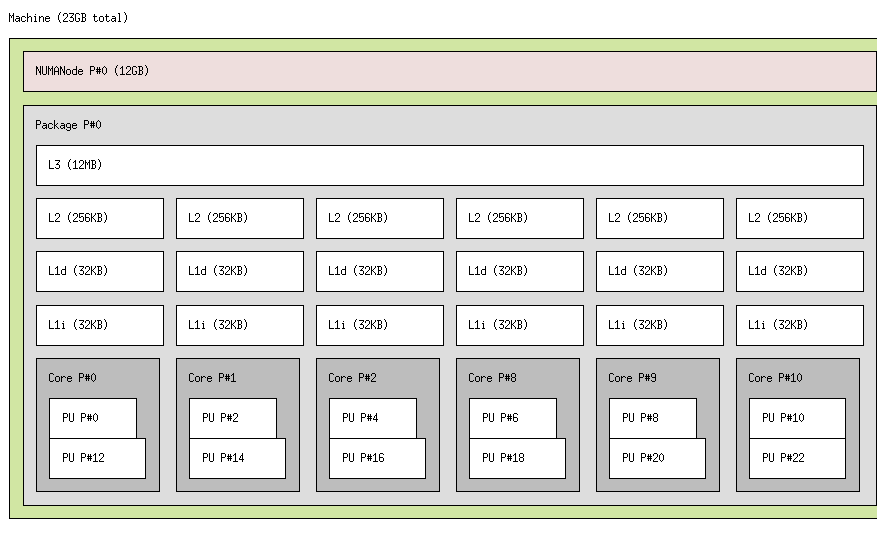
\includegraphics[width=14cm]{fig1.png}
\end{center}

\section*{Timing sequential and parallel executions}

\item[] 2. Describe what do you need to add to your program to measure the elapsed execution time between a pair of points in the program, clearly indicating the library header file that needs to be included, the library functions that need to be invoked, the data structure and its fields.


\begin{itemize}

\item[] To measure the time we need to get a timestamp with the time of the day when the execution starts and subtract that value to the time of day when the program ends. To do so we use the following:

\item The library:
\begin{lstlisting}[style=CStyle]
	#include <sys/time.h>
\end{lstlisting}

\item The function:
\begin{lstlisting}[style=CStyle]
	int  gettimeofday(struct timeval *, void *);
\end{lstlisting}

\item The data structure \textbf{timeval}, which includes the following fields:

\begin{lstlisting}[style=CStyle]
	time_t         tv_sec      seconds
	suseconds_t    tv_usec     microseconds
\end{lstlisting}





\end{itemize}




\item[] 3. Plot the speed–up obtained when varying the number of threads (strong scalability) and problemsize (weak scalability) for pi omp.c. Reason about how the scalability of the program.

\begin{figure}[H]%
\centering
\subfloat{{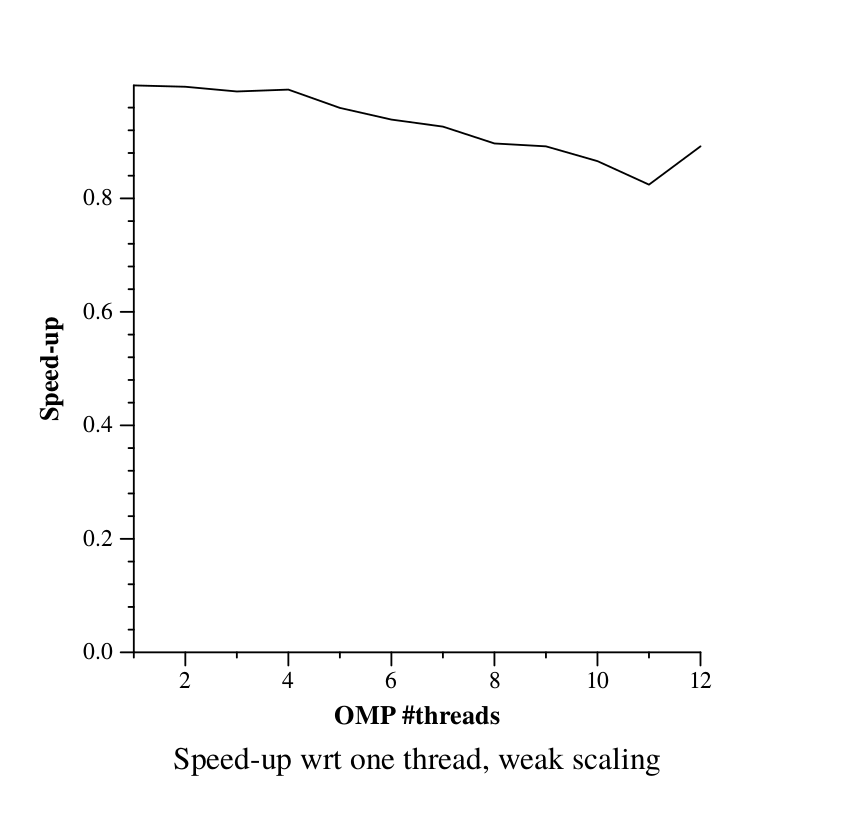
\includegraphics[width=6cm]{weak.png} }}%
\qquad
\subfloat{{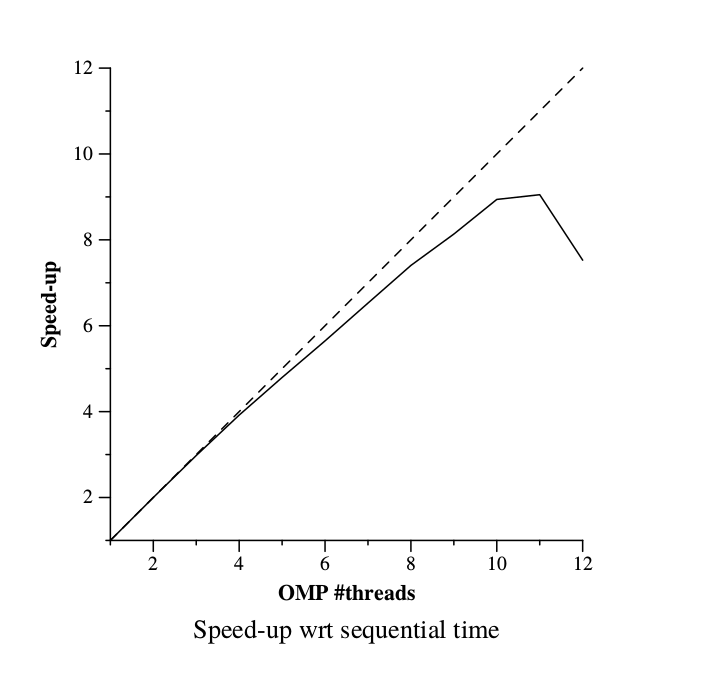
\includegraphics[width=6cm]{strong.png} }}%
\end{figure}
\begin{itemize}
\item[] When we are in weak scalability, the speedup does not change so much, it means the scalability is good and we can keep increasing the problem size while increasing the threads and the execution time will not be much greater. In the case of strong scalability, we can see that more than 11 threads start to decrease the speed-up, so it does not have a great strong scalability, with 11 as the optimal number of threads.
\end{itemize}

\section*{Visualizing the task graph and data dependences}


\item[] 4. Include the source code for function dot product in which you show the Tareador instrumentation that has been added to study the potential parallelism in the code. This instrumentation has to appropriately define tasks and filter the analysis of variable(s) that cause the dependence(s).

%this is too long, better include the code to the archive
%\lstinputlisting[caption=Scheduler, style=CStyle]{dot_product.c}
\begin{itemize}
	\item[] The source code has been added to the archive and is named dot\_product.c
\end{itemize}

\item[] 5. Capture the task dependence graph for that task decomposition and the execution timelines (for 8 processors) that allow you to understand the potential parallelism attainable. Briefly comment the relevant information that is reported by the tools.

\begin{figure}[H]%
\centering
\subfloat{{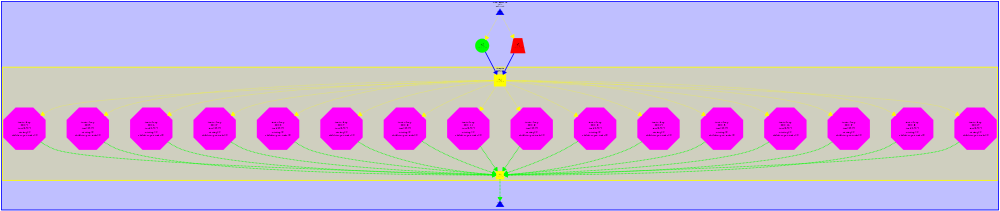
\includegraphics[width=18cm]{graph.png} }}%
\label{fig:test}%
\end{figure}
\begin{figure}[H]%
\centering
\subfloat{{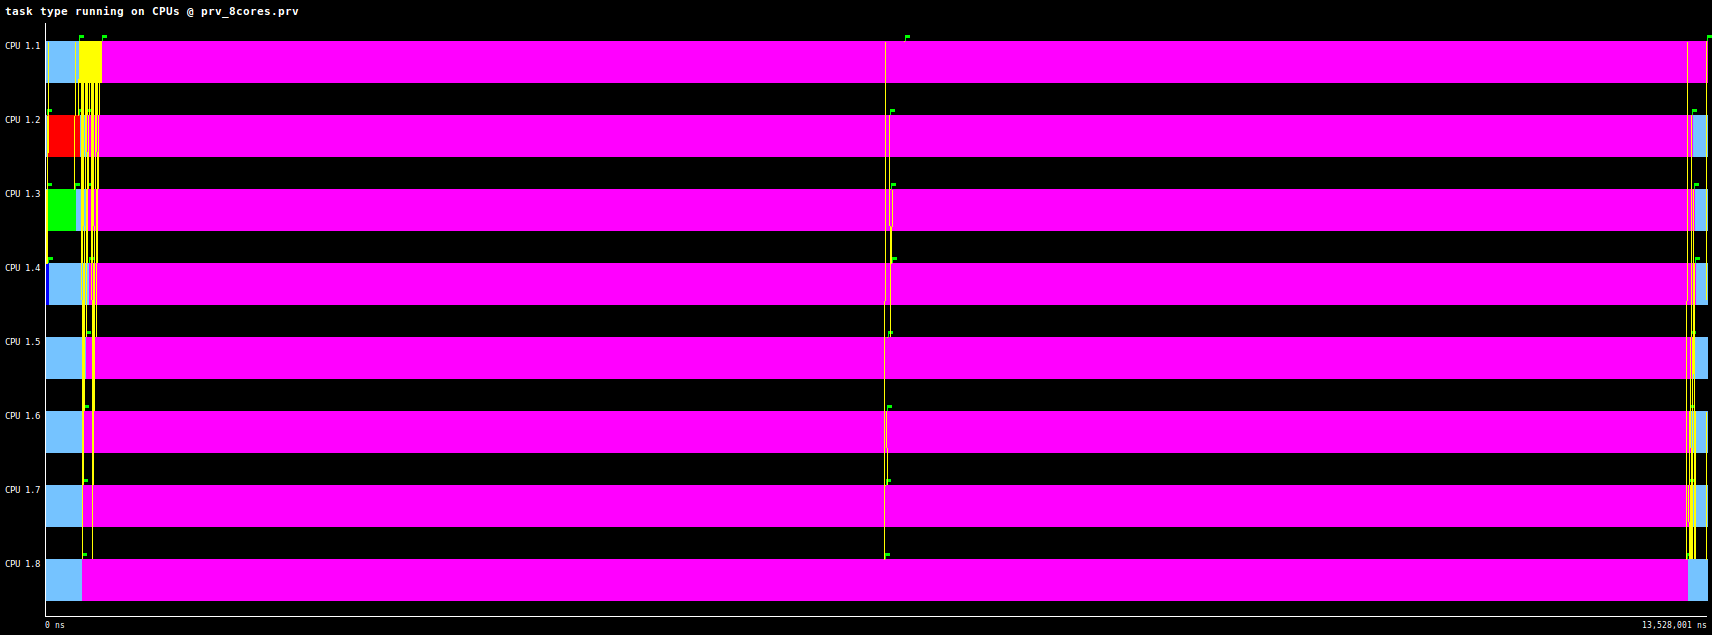
\includegraphics[width=18cm]{timelines.png} }}%
\end{figure}





\section*{Analysis of task decompositions}

\item[] 6. Complete the following table for the initial and different versions generated for 3dfft\_seq.c, briefly
commenting the evolution of the metrics with the different versions.
\begin{center}
\begin{tabular}{| c || c | c | c | }
  \hline
  \textbf{Version} & $T_1$ & $T_{\infty}$ & \textbf{Parallelism}\\ \hline \hline
  seq & 593772 & 593758 & 1.000\\ \hline
  v1 & 593772 & 593758 & 1.000\\ \hline
  v2  & 594054 & 315537 & 1.883 \\ \hline
  v3  &  594054 & 108701 & 5.465\\ \hline
  v4  & 594054 & 59694 & 9.952 \\
  \hline

\end{tabular}
\end{center}



\item[] 7. With the results from the parallel simulation with 2, 4, 8, 16 and 32 processors, draw the execution
time and speedup plots for version v4 with respect to the sequential execution (that you can
estimate from the simulation of the initial task decomposition that we provided in 3dfft seq.c,
using just 1 processor). Briefly comment the scalability behaviour shown on these two plots.


\begin{figure}[H]%
\centering
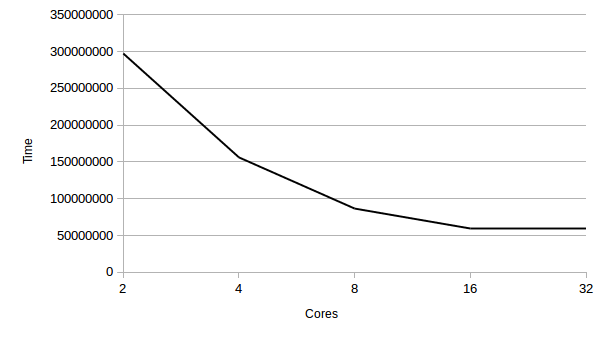
\includegraphics[width=9cm]{plotTimeCores.png}
\caption{Execution time in ns }
\label{fig:test}%
\end{figure}
\begin{figure}[H]
\centering
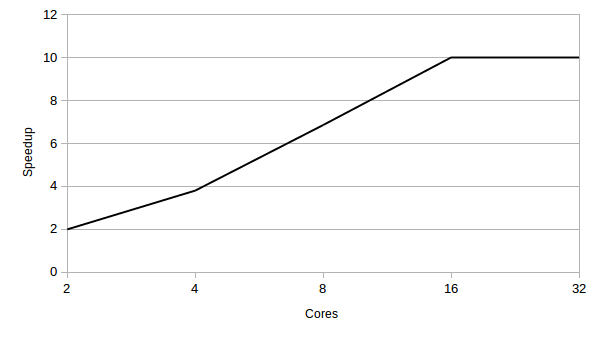
\includegraphics[width=9cm]{plotSpeedup.png}
\caption{Speedup v4 vs. seq}
\label{fig:Speedup plot}%
\end{figure}



\section* {Tracing sequential and parallel executions}


\item[] 8. From the instrumented version of pi seq.c, and using the appropriate Paraver configuration
file, obtain the value of the parallel fraction φ for this program when executed with 100.000.000
iterations, showing the steps you followed to obtain it. Clearly indicate which Paraver configuration
file(s) did you use.



\item[] 9. From the instrumented version of pi omp.c, and using the appropriate Paraver configuration file,
show a profile of the \% of time spent in the different OpenMP states when using 8 threads and for
100.000.000 iterations. Clearly indicate which Paraver configuration file(s) did you use and your
own conclusions from that profile.




\end{enumerate}
\end{document}